\chapter{Decision-Theoretic Planning}
\label{ch:background}
% Introduction on what is Decision-Theoretic Planning
Automated sequential decision making comprises the central problem of planning under uncertainty. 
\textit{Decision-theoretic planning} (DTP) is concerned with the design of plans or \textit{policies} for settings in which uncertainty exists about the effects of actions, where the decision maker or \textit{agent} has incomplete information about the environment and its initial conditions, and trade-offs need to be made between potentially conflicting objectives to determine an optimal course of action.
% ?
% Chapter organized as follows: section x....

\section{General Problem Formulation}
\label{sec:problem-formulation}
% Formulation of what kind of planning problems are considered in Decision-Theoretic Planning

The class of problems that are considered in decision-theoretic planning are those that require optimal stochastic control through the actions of decision maker(s), referred to as \textit{agent(s)}, in systems whose dynamics can be modeled as \textit{stochastic processes} \cite{Boutilier1999}.
The agent(s) in these systems sequentially need to choose from a set of actions that influence the system's behavior, consequently making the system switch from one state to another.
In these settings the system's current state and the agent's choice of action determines the probability distribution over the states the system might reach next.
In addition, the agent(s) might be uncertain about the system's current state, implying the need to infer from observations and making decisions based on probabilistic estimates of the system's state.

Typically the problems under consideration involve certain objectives to be achieved (e.g., tasks to be fulfilled) or properties to be satisfied (e.g., avoiding certain system states). 
Therefore the agent should decide on a optimal plan or \textit{policy} which makes it most likely for the system to reach its targets, while minimizing the risk of producing undesirable states and the accompanied costs of the policy.
To find such a policy for sequential decision-making problems, a typical approach is to first setup a probabilistic model of the system and then apply a decision-theoretic planning algorithm on this model.
This probabilistic model comprises a system representation which defines the state space in terms of a set of multi-valued features, the set of actions for the agent to select together with the associated uncertainty defined by transition-probabilities, and a goal specification or performance metric regularly expressed by means of a reward structure.

Overall decision-theoretic planning aims to devise planning algorithms for planning under uncertainty, a problem that is addressed in numerous different fields of research such as AI planning and control theory.
In particular difficulties arise when planning techniques are applied to determine courses of action for real-world settings, such as 

\section{System Representations: Markov Models}
\label{sec:system-representation}

%

\subsection{Markov Chains}
\label{subsec:markov-chains}
% Markov Chains: States and Transitions

%

\subsection{Hidden Markov Models}
\label{subsec:hidden-markov-models}
% Hidden Markov Models: Observations (partially observable)

%

\subsection{Markov Decision Processes}
\label{subsec:mdps}

% MDPs: Actions --> Is a probabilistic model			% Driven by the actions of an agent
% 	(Exogeneous) events
% Policies

%

\subsection{Partially Observable MDPs}
\label{subsec:pomdps}

% Observations: .. POMDP
% Reward Models and Value Functions

% 

\section{Learning Optimal Policies}
\label{sec:planning}

% 

\subsection{Model-Free Planning Techniques}
\label{subsec:model-free-planning}

% 

\subsection{Model-Based Planning Techniques}
\label{subsec:model-based-planning}

\begin{figure}[ht!]
	\centering
	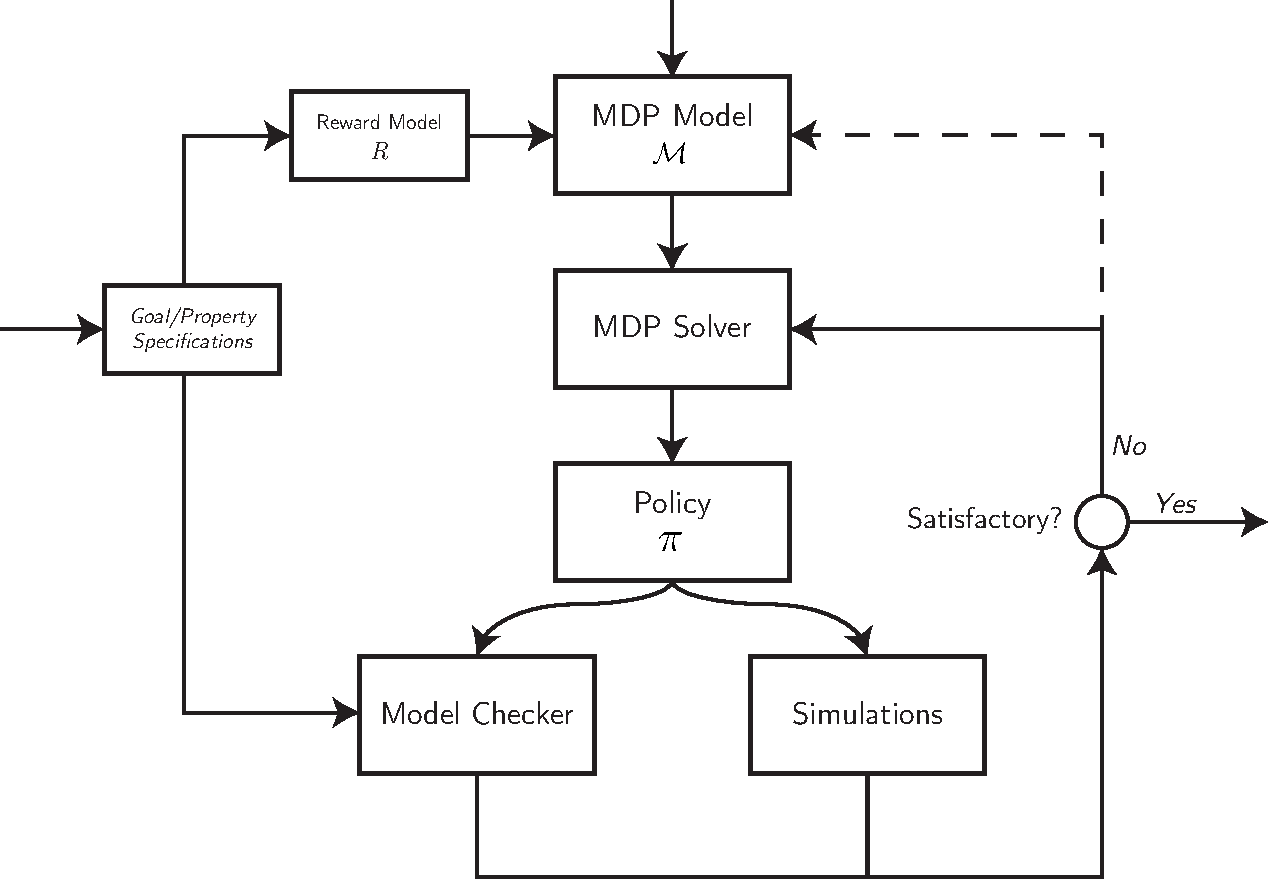
\includegraphics[width=\textwidth]{mdp-planning-diagram}
	\caption{Block diagram of the embedded system's overall software architecture.}
	\label{fig:architecture}
\end{figure}
% Planning algorithms for MDPs
% Planning algorithms for POMDPs

% 










% perceptual aliasing!!!!!!